\section{Mockups}
In questa sezione vengono presentati i principali mockup dell'interfaccia utente dell'applicativo \textbf{JavaBrew}. I mockup rappresentano le principali schermate dell'applicazione e forniscono una panoramica intuitiva delle funzionalità offerte agli utenti delle diverse tipologie (admin, worker, user).

\subsection{Login}
\begin{figure}[H]
    \centering
    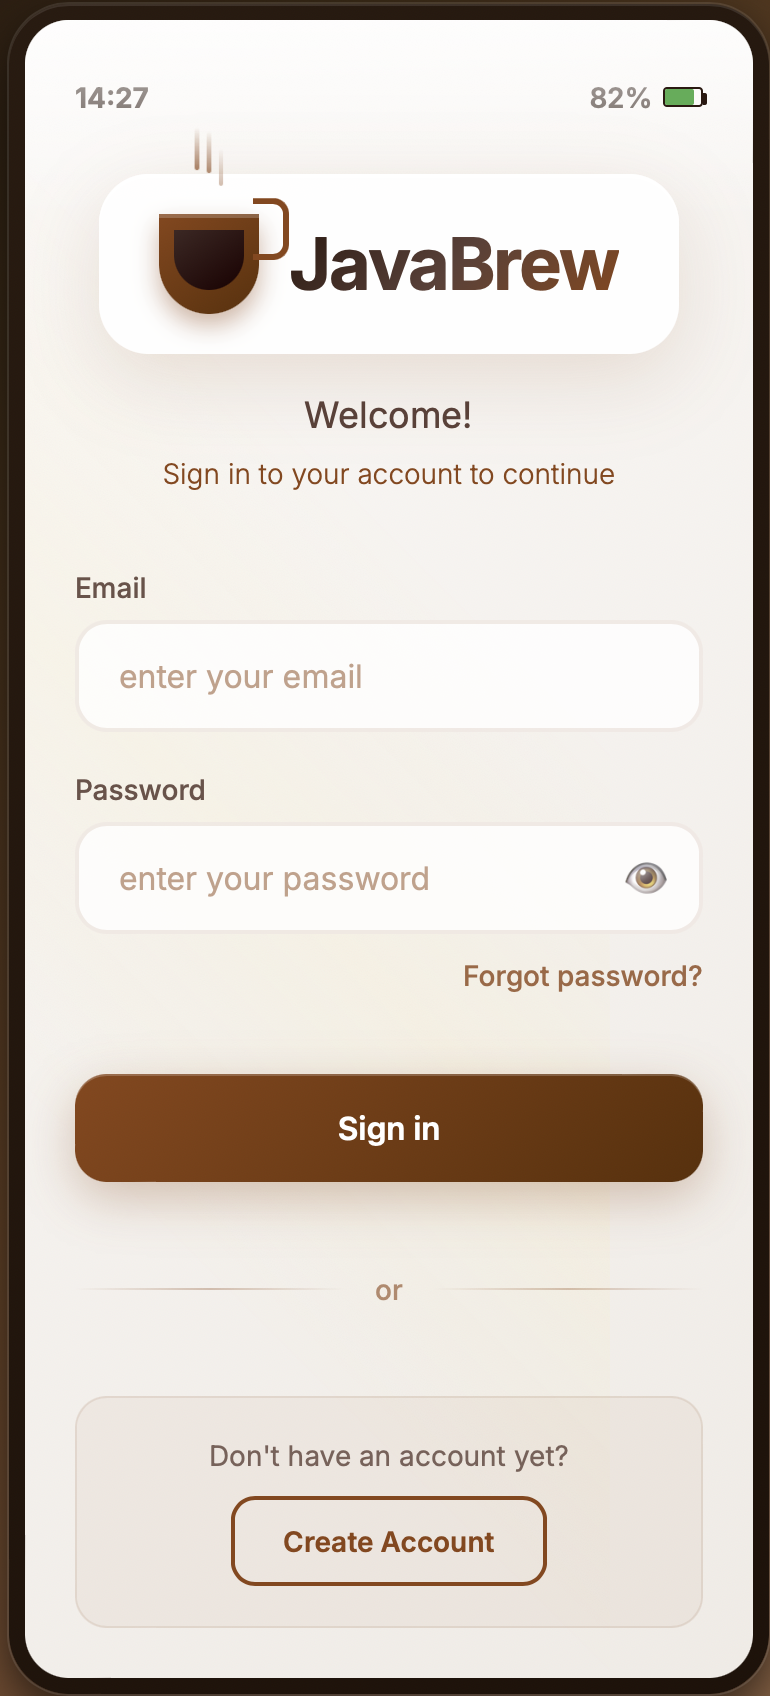
\includegraphics[width=0.5\textwidth]{./assets/login.png}
    \caption{Schermata di login.}
\end{figure}
La schermata di login permette agli utenti di autenticarsi tramite le proprie credenziali (username e password). Sono disponibili anche le opzioni per l’accesso come amministratore e per la registrazione di un nuovo account.

\subsection{Registrazione}
\begin{figure}[H]
    \centering
    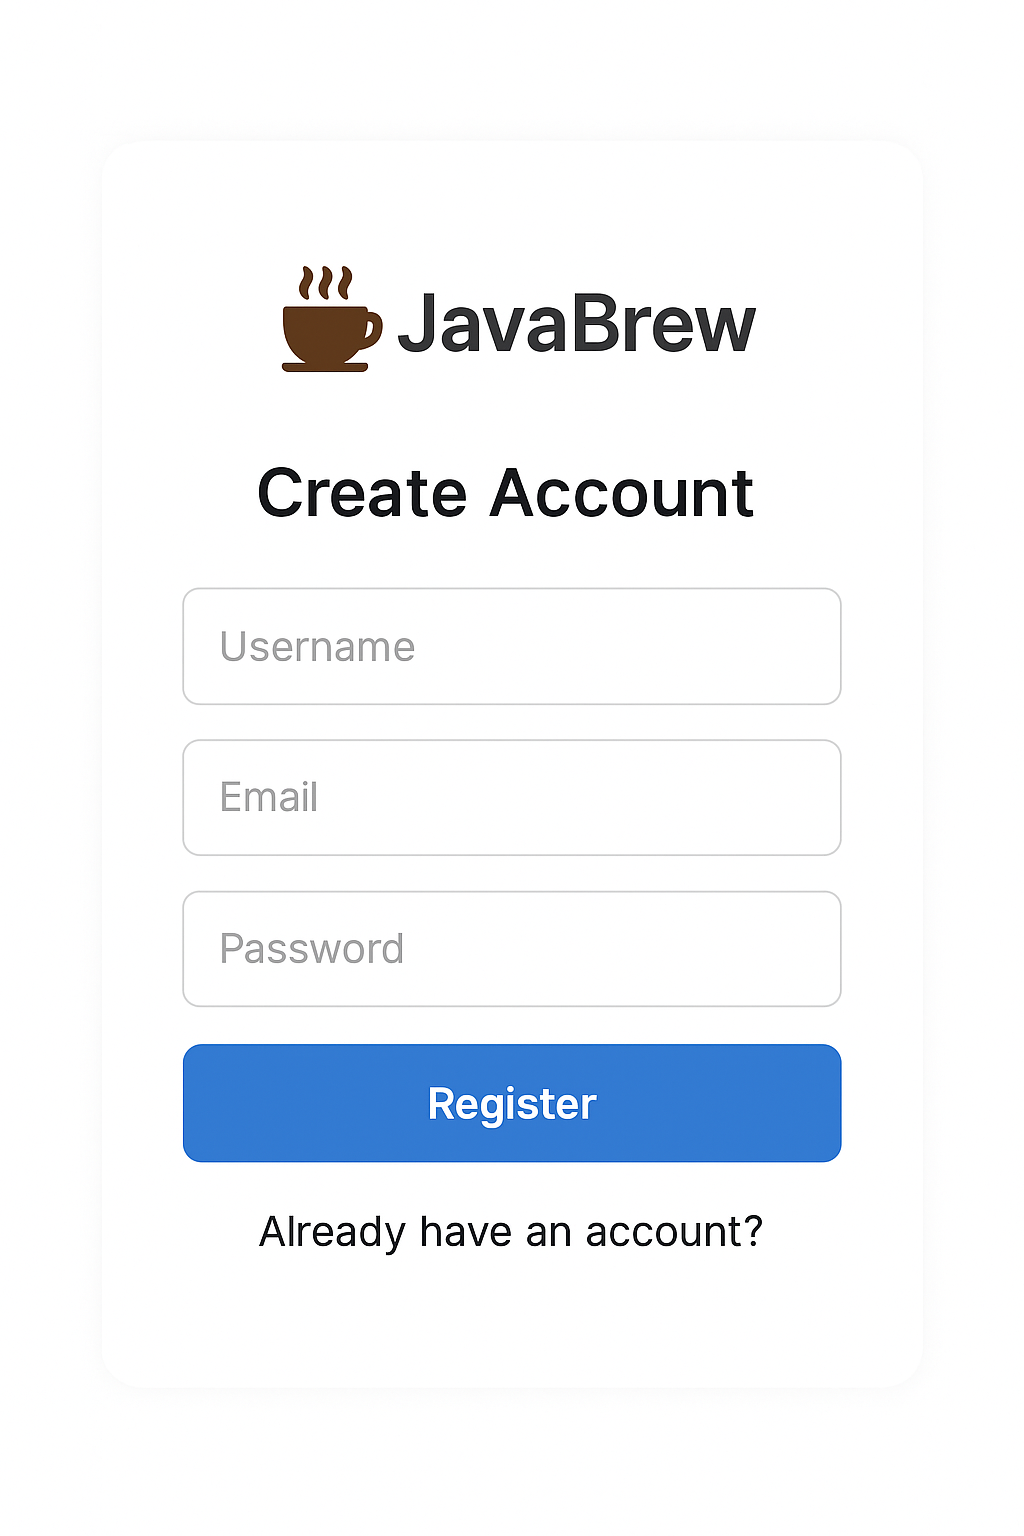
\includegraphics[width=0.5\textwidth]{./assets/Create_acoount.png}
    \caption{Schermata di registrazione.}
\end{figure}
Nella schermata di registrazione l’utente può creare un nuovo account inserendo username, email e password.

\subsection{Dashboard Admin}
\begin{figure}[H]
    \centering
    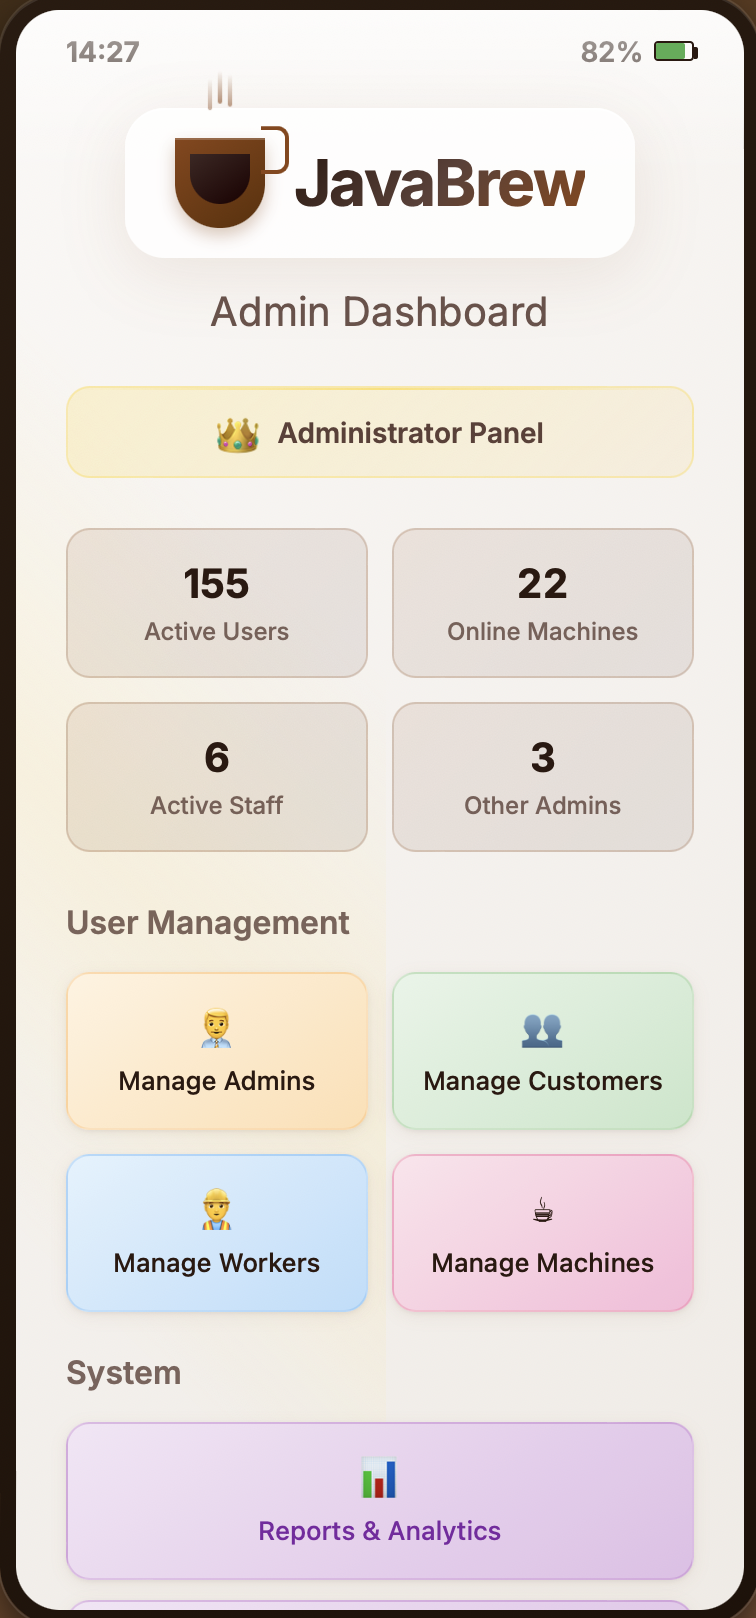
\includegraphics[width=0.5\textwidth]{./assets/admin.png}
    \caption{Dashboard per amministratore.}
\end{figure}
L’admin ha accesso a funzionalità avanzate: aggiunta/gestione macchinette, visualizzazione analytics di vendita, gestione prodotti e gestione utenti (aggiunta, ricerca, rimozione).


\subsection{Customer Dashboard}
\begin{figure}[H]
    \centering
    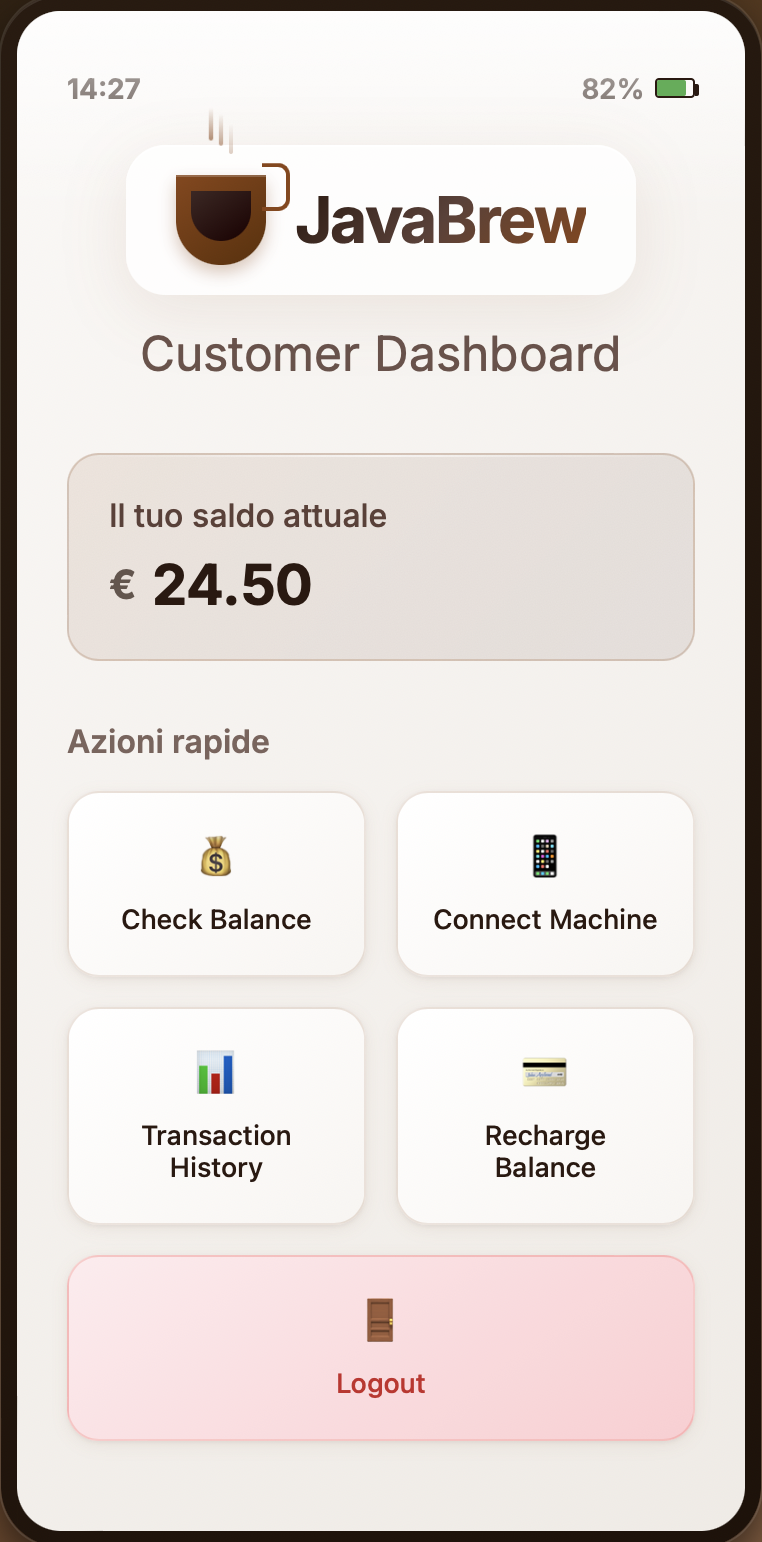
\includegraphics[width=0.4\textwidth]{./assets/customer.png}
    \caption{Dashboard utente standard.}
\end{figure}
Nella dashboard customer sono disponibili le funzioni di selezione prodotto e ricarica del saldo, principali azioni per l’utente finale.

\subsection{Worker Dashboard}
\begin{figure}[H]
    \centering
    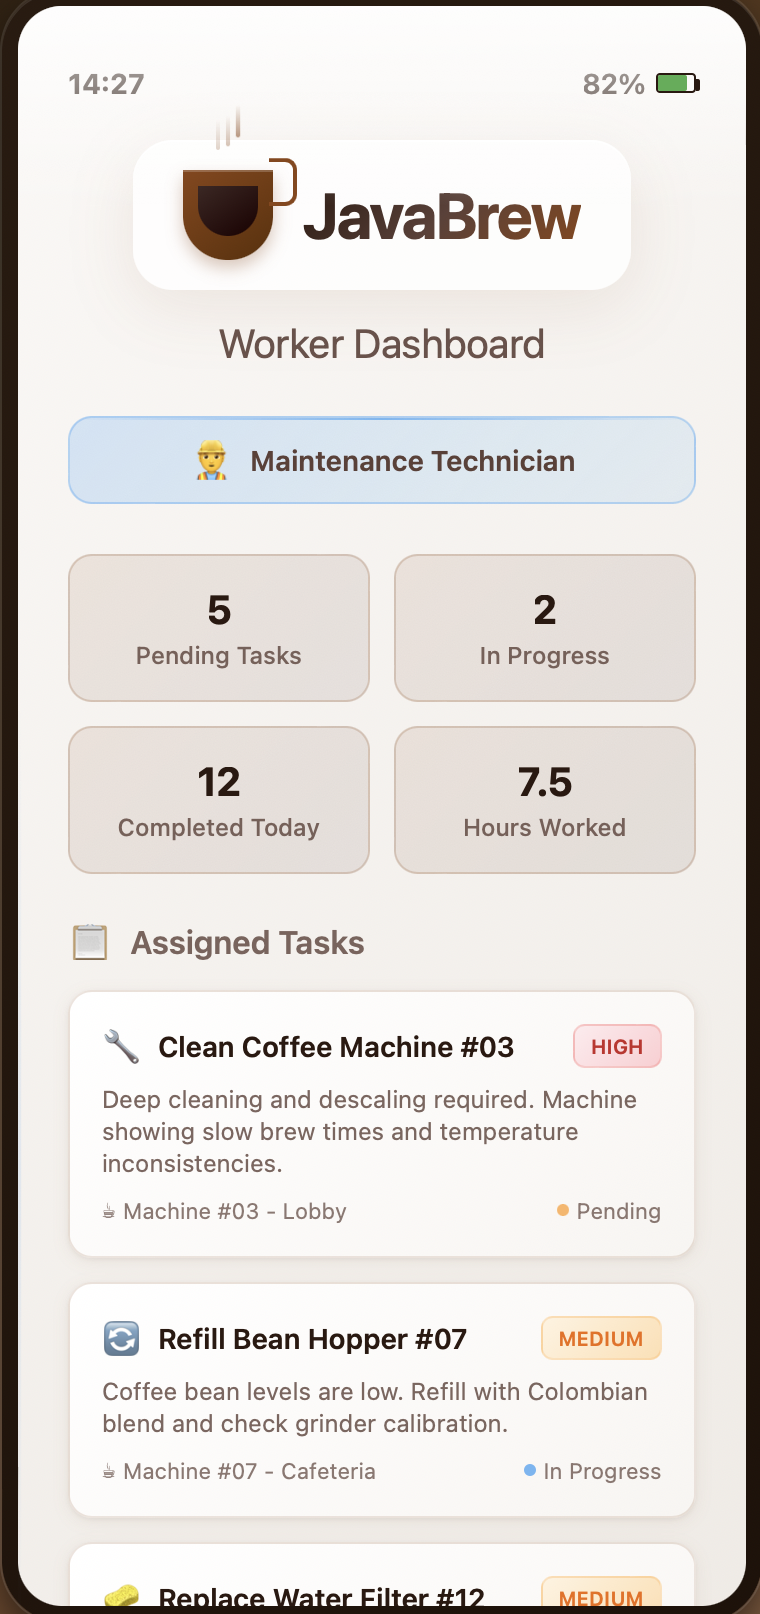
\includegraphics[width=0.4\textwidth]{./assets/worker.png}
    \caption{Dashboard per il lavoratore.}
\end{figure}
Il lavoratore ha accesso a funzionalità di gestione delle macchinette, come la visualizzazione dello stato delle macchine e la possibilità di rifornirle con nuovi prodotti.
\subsection{Items}  
\begin{figure}[H]
    \centering
    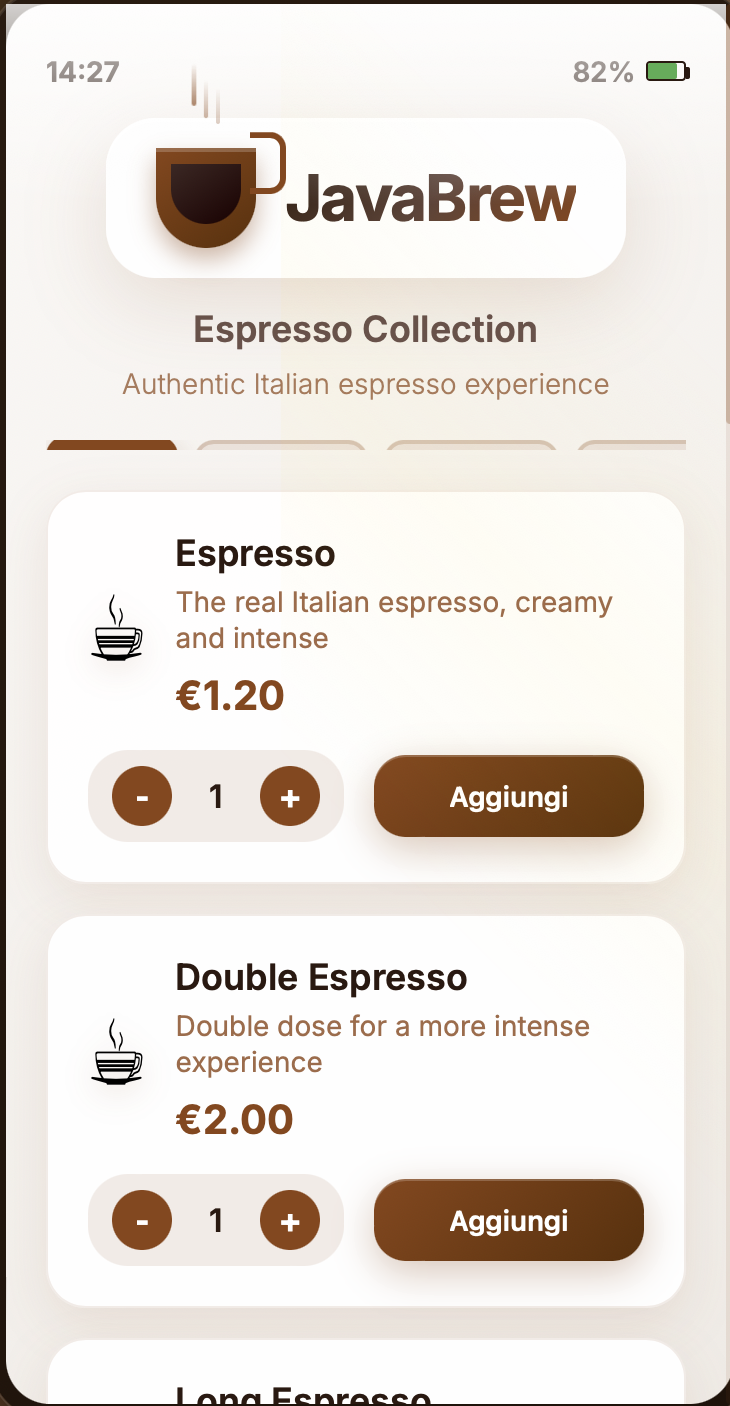
\includegraphics[width=0.4\textwidth]{./assets/items.png}
    \caption{Schermata di gestione degli articoli.}
\end{figure}
Nella schermata di elenco degli articoli, il cliente può visualizzare i prodotti disponibili, con la possibilità di aggiungerli al carrello per l'acquisto. 